\documentclass[11pt,portuguese,]{article}
\usepackage{lmodern}
\usepackage{amssymb,amsmath}
\usepackage{ifxetex,ifluatex}
\usepackage{fixltx2e} % provides \textsubscript
\ifnum 0\ifxetex 1\fi\ifluatex 1\fi=0 % if pdftex
  \usepackage[T1]{fontenc}
  \usepackage[utf8]{inputenc}
\else % if luatex or xelatex
  \ifxetex
    \usepackage{mathspec}
  \else
    \usepackage{fontspec}
  \fi
  \defaultfontfeatures{Ligatures=TeX,Scale=MatchLowercase}
    \setmainfont[]{times}
\fi
% use upquote if available, for straight quotes in verbatim environments
\IfFileExists{upquote.sty}{\usepackage{upquote}}{}
% use microtype if available
\IfFileExists{microtype.sty}{%
\usepackage{microtype}
\UseMicrotypeSet[protrusion]{basicmath} % disable protrusion for tt fonts
}{}
\usepackage[margin=1in]{geometry}
\usepackage{hyperref}
\hypersetup{unicode=true,
            pdftitle={PIB 2º Trimestre de 2018},
            pdfauthor={Arthur Welle; Gabriel Mandarino; Gabriel Petrini},
            pdfborder={0 0 0},
            breaklinks=true}
\urlstyle{same}  % don't use monospace font for urls
\ifnum 0\ifxetex 1\fi\ifluatex 1\fi=0 % if pdftex
  \usepackage[shorthands=off,main=portuguese]{babel}
\else
  \usepackage{polyglossia}
  \setmainlanguage[]{portuguese}
\fi
\usepackage{longtable,booktabs}
\usepackage{graphicx,grffile}
\makeatletter
\def\maxwidth{\ifdim\Gin@nat@width>\linewidth\linewidth\else\Gin@nat@width\fi}
\def\maxheight{\ifdim\Gin@nat@height>\textheight\textheight\else\Gin@nat@height\fi}
\makeatother
% Scale images if necessary, so that they will not overflow the page
% margins by default, and it is still possible to overwrite the defaults
% using explicit options in \includegraphics[width, height, ...]{}
\setkeys{Gin}{width=\maxwidth,height=\maxheight,keepaspectratio}
\IfFileExists{parskip.sty}{%
\usepackage{parskip}
}{% else
\setlength{\parindent}{0pt}
\setlength{\parskip}{6pt plus 2pt minus 1pt}
}
\setlength{\emergencystretch}{3em}  % prevent overfull lines
\providecommand{\tightlist}{%
  \setlength{\itemsep}{0pt}\setlength{\parskip}{0pt}}
\setcounter{secnumdepth}{0}
% Redefines (sub)paragraphs to behave more like sections
\ifx\paragraph\undefined\else
\let\oldparagraph\paragraph
\renewcommand{\paragraph}[1]{\oldparagraph{#1}\mbox{}}
\fi
\ifx\subparagraph\undefined\else
\let\oldsubparagraph\subparagraph
\renewcommand{\subparagraph}[1]{\oldsubparagraph{#1}\mbox{}}
\fi

%%% Use protect on footnotes to avoid problems with footnotes in titles
\let\rmarkdownfootnote\footnote%
\def\footnote{\protect\rmarkdownfootnote}

%%% Change title format to be more compact
\usepackage{titling}

% Create subtitle command for use in maketitle
\newcommand{\subtitle}[1]{
  \posttitle{
    \begin{center}\large#1\end{center}
    }
}

\setlength{\droptitle}{-2em}

  \title{PIB 2º Trimestre de 2018}
    \pretitle{\vspace{\droptitle}\centering\huge}
  \posttitle{\par}
    \author{Arthur Welle \\ Gabriel Mandarino \\ Gabriel Petrini}
    \preauthor{\centering\large\emph}
  \postauthor{\par}
      \predate{\centering\large\emph}
  \postdate{\par}
    \date{14 de setembro de 2018}


\begin{document}
\maketitle

\section{PIB}\label{pib}

\subsection[Tabela Resumo]{\texorpdfstring{Tabela Resumo\footnote{Variação
  percentual calculada a partir da série encadeada a preços de 1995 com
  ajuste sazonal.}}{Tabela Resumo}}\label{tabela-resumo1}

\begin{longtable}[]{@{}lrrrrr@{}}
\caption{Resultados PIB a preços de mercado}\tabularnewline
\toprule
& 2017 Q2 & 2017 Q3 & 2017 Q4 & 2018 Q1 & 2018 Q2\tabularnewline
\midrule
\endfirsthead
\toprule
& 2017 Q2 & 2017 Q3 & 2017 Q4 & 2018 Q1 & 2018 Q2\tabularnewline
\midrule
\endhead
Acum. ano & 0,2 & 0,6 & 1,0 & 1,2 & 1,1\tabularnewline
Acum. 4 trim. & -1,2 & -0,2 & 1,0 & 1,3 & 1,4\tabularnewline
Ano ant. & 0,4 & 1,4 & 2,1 & 1,2 & 1,0\tabularnewline
Trim. ant. & 0,4 & 0,6 & 0,0 & 0,1 & 0,2\tabularnewline
\bottomrule
\end{longtable}

\subsection{Trimestre / trimestre imediatamente anterior (com ajuste
sazonal)}\label{trimestre-trimestre-imediatamente-anterior-com-ajuste-sazonal}

\begin{center}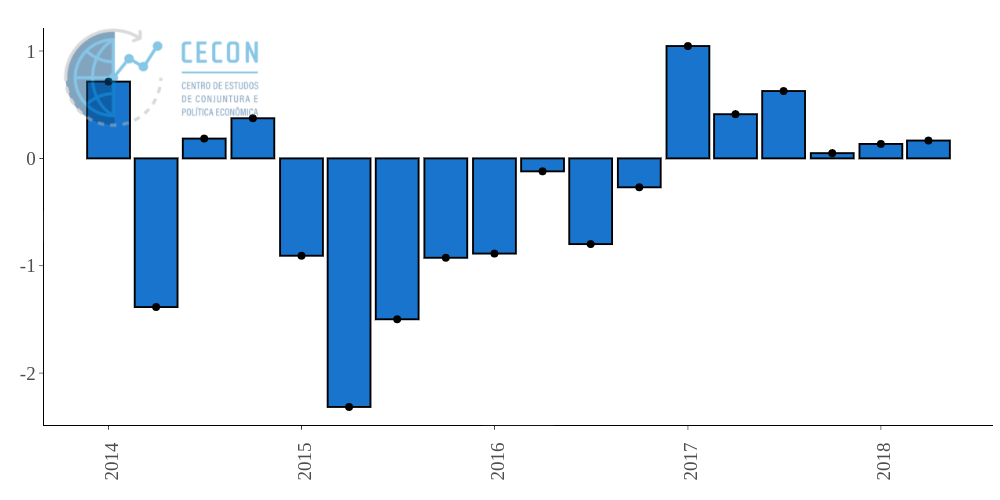
\includegraphics[width=1\linewidth]{Grafico_PIB} \end{center}

\section{PIB Setorial}\label{pib-setorial}

\subsection[Tabela Resumo - Oferta]{\texorpdfstring{Tabela Resumo -
Oferta\footnote{Variação percentual calculada a partir da série
  encadeada a preços de 1995 com ajuste sazonal.}}{Tabela Resumo - Oferta}}\label{tabela-resumo---oferta2}

\begin{longtable}[]{@{}lrrrr@{}}
\caption{Tabela resumo - Oferta}\tabularnewline
\toprule
& Agropecuária & Indústria & Serviços & PIB\tabularnewline
\midrule
\endfirsthead
\toprule
& Agropecuária & Indústria & Serviços & PIB\tabularnewline
\midrule
\endhead
Valor anterior & 1,30 & 0,1 & 0,1 & 0,1\tabularnewline
Último Valor & 0,04 & -0,6 & 0,3 & 0,2\tabularnewline
12 meses anteriores & -2,5 & -0,3 & 0,7 & 0,4\tabularnewline
Variação percentual & 1,3\% & 0,2\% & 0,6\% & 0,3\%\tabularnewline
Taxa acumulada & -0,6 & 1 & 1 & 0,98\tabularnewline
Taxa anualizada & 0,5 & -7 & 4 & 2\tabularnewline
\bottomrule
\end{longtable}

\subsection{Comparação trimestral -
Oferta}\label{comparacao-trimestral---oferta}

\begin{center}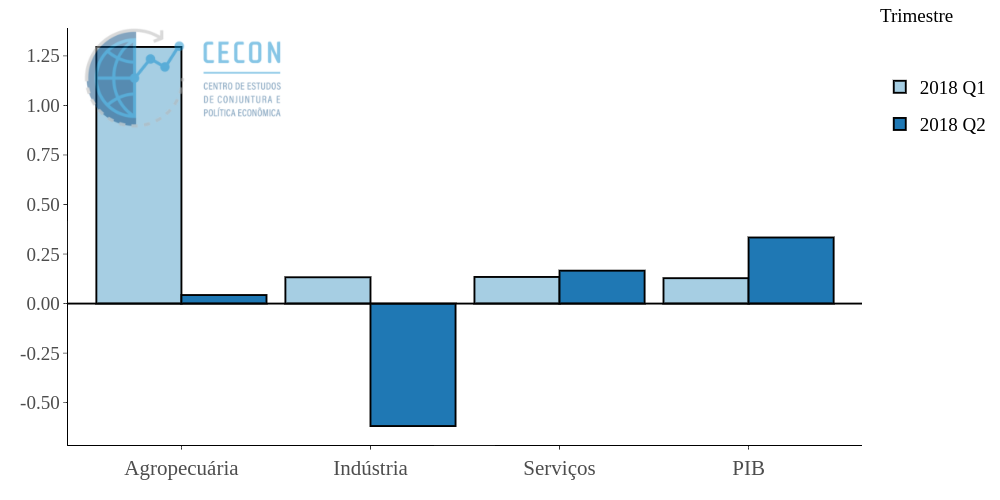
\includegraphics[width=1\linewidth]{Grafico_Setores} \end{center}

\subsection{Decomposição - Oferta}\label{decomposicao---oferta}

\begin{longtable}[]{@{}lrrrrr@{}}
\caption{Contribuição ao PIB - Oferta}\tabularnewline
\toprule
& 2017 Q2 & 2017 Q3 & 2017 Q4 & 2018 Q1 & 2018 Q2\tabularnewline
\midrule
\endfirsthead
\toprule
& 2017 Q2 & 2017 Q3 & 2017 Q4 & 2018 Q1 & 2018 Q2\tabularnewline
\midrule
\endhead
Agropecuária & -0,18 & -0,13 & 0,00 & 0,09 & 0,00\tabularnewline
Indústria & -0,05 & 0,17 & 0,13 & 0,03 & -0,12\tabularnewline
Serviços & 0,42 & 0,34 & 0,08 & 0,08 & 0,20\tabularnewline
PIB & 0,41 & 0,62 & 0,05 & 0,13 & 0,17\tabularnewline
\bottomrule
\end{longtable}

\subsection{Agropecuária}\label{agropecuaria}

\begin{center}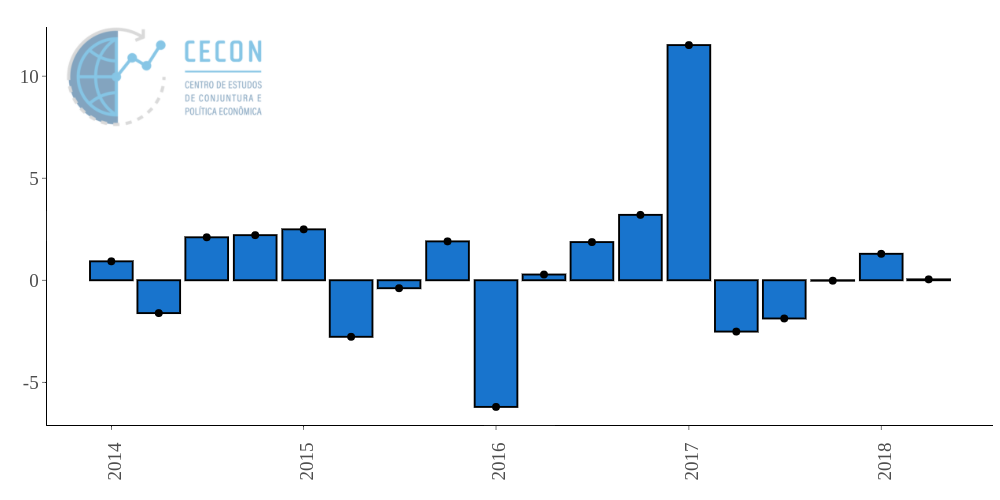
\includegraphics[width=1\linewidth]{Grafico_Agro} \end{center}

\subsection{Indústria}\label{industria}

\begin{center}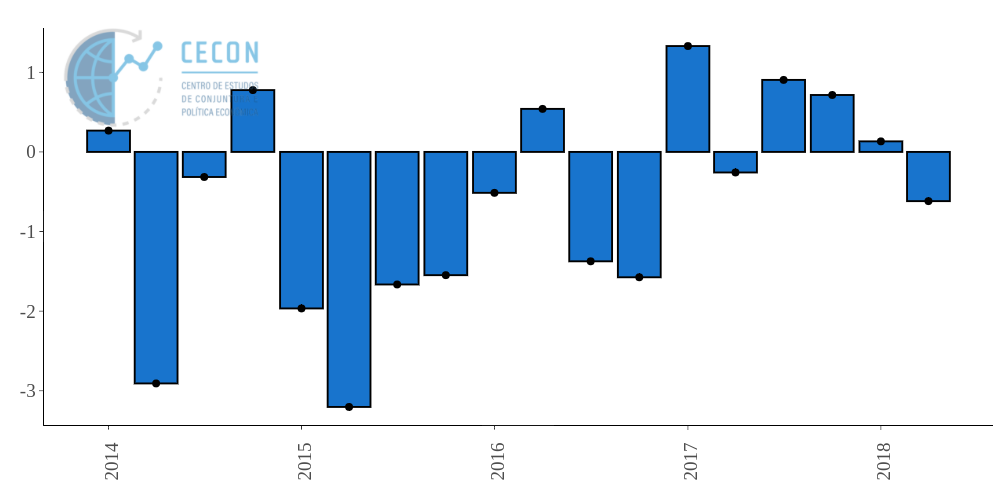
\includegraphics[width=1\linewidth]{Grafico_Industria} \end{center}

\subsection{Serviços}\label{servicos}

\begin{center}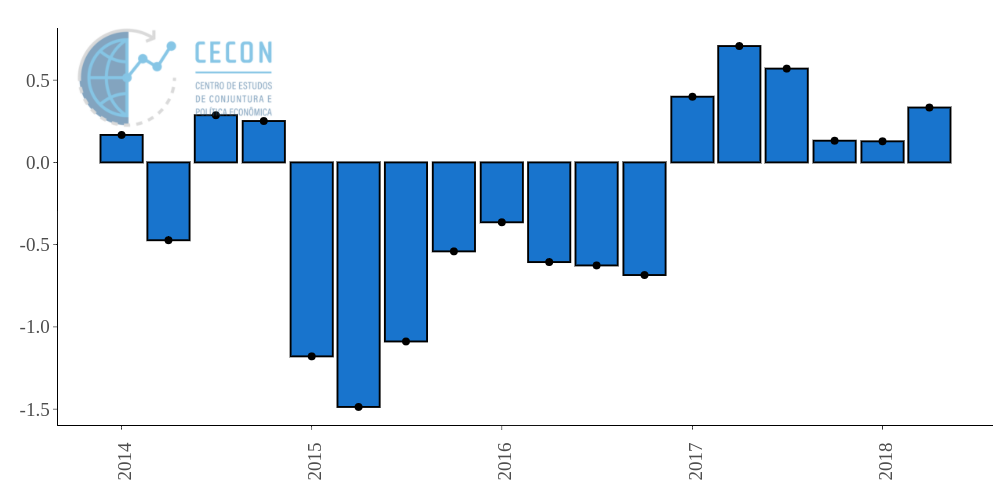
\includegraphics[width=1\linewidth]{Grafico_Servicos} \end{center}

\section{Valor Adicionado}\label{valor-adicionado}

\subsection[Valor Adicionado - Resumo]{\texorpdfstring{Valor Adicionado
- Resumo\footnote{Variação percentual calculada a partir da série
  encadeada a preços de 1995 com ajuste sazonal.}}{Valor Adicionado - Resumo}}\label{valor-adicionado---resumo3}

\begin{longtable}[]{@{}lrr@{}}
\caption{Tabela resumo - Valor Adicionado}\tabularnewline
\toprule
& Valor Adicionado & PIB\tabularnewline
\midrule
\endfirsthead
\toprule
& Valor Adicionado & PIB\tabularnewline
\midrule
\endhead
Valor anterior & 0,11 & 0,17\tabularnewline
12 meses anteriores & 0,13 & 0,41\tabularnewline
Variação percentual & 0,65\% & 0,35\%\tabularnewline
Taxa acumulada & 0,89 & 0,98\tabularnewline
Taxa anualizada & 1,3 & 2\tabularnewline
\bottomrule
\end{longtable}

\subsection{Valor Adicionado}\label{valor-adicionado-1}

\begin{center}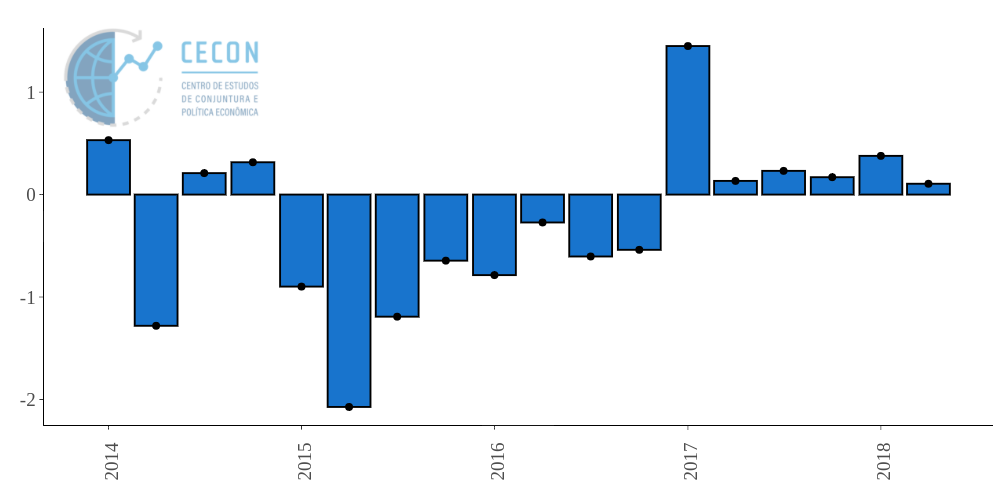
\includegraphics[width=1\linewidth]{Grafico_VA} \end{center}

\section{Demanda}\label{demanda}

\subsection[Tabela Resumo - Demanda]{\texorpdfstring{Tabela Resumo -
Demanda\footnote{Variação percentual calculada a partir da série
  encadeada a preços de 1995 com ajuste sazonal.}}{Tabela Resumo - Demanda}}\label{tabela-resumo---demanda4}

\begin{longtable}[]{@{}lrrrrrr@{}}
\caption{Tabela resumo - Demanda}\tabularnewline
\toprule
& Fam & Gov & FBCF & Exp & Imp & PIB\tabularnewline
\midrule
\endfirsthead
\toprule
& Fam & Gov & FBCF & Exp & Imp & PIB\tabularnewline
\midrule
\endhead
Valor anterior & 0,07 & 0,49 & -1,85 & -5,46 & -2,12 &
0,17\tabularnewline
12 meses anteriores & 1,23 & -0,33 & 0,89 & 2 & -1,48 &
0,41\tabularnewline
Variação percentual & 0,4\% & 0,3\% & 0,2\% & -4,8\% & 0,6\% &
0,3\%\tabularnewline
Taxa acumulada & 1,7 & 0,054 & 2,2 & -2,5 & 7 & 0,98\tabularnewline
Taxa anualizada & 0,81 & 6 & -20 & -49 & -23 & 2\tabularnewline
\bottomrule
\end{longtable}

\subsection{Comparação trimestral -
Demanda}\label{comparacao-trimestral---demanda}

\begin{center}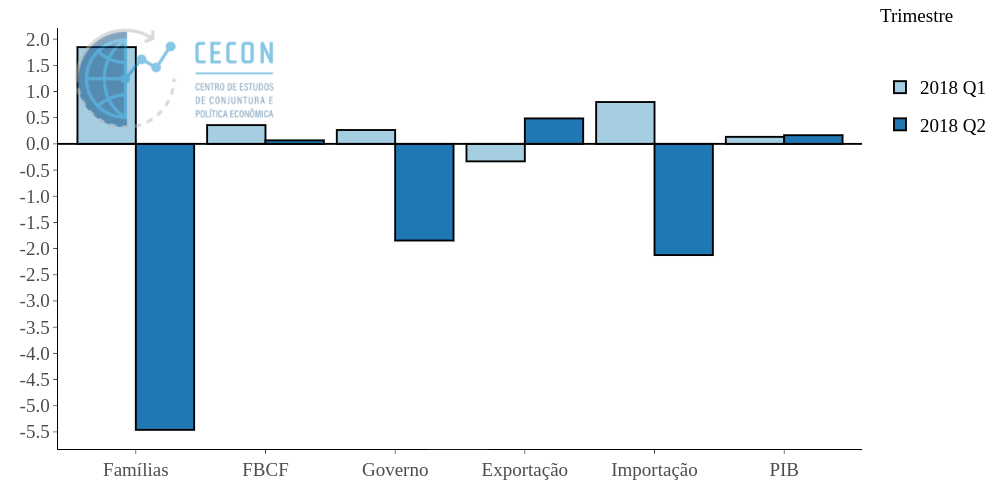
\includegraphics[width=1\linewidth]{Grafico_Demanda} \end{center}

\subsection{Decomposição - Demanda}\label{decomposicao---demanda}

\begin{longtable}[]{@{}lrrrrr@{}}
\caption{Contribuição ao PIB - Demanda (sem variação de
estoques)}\tabularnewline
\toprule
& 2017 Q2 & 2017 Q3 & 2017 Q4 & 2018 Q1 & 2018 Q2\tabularnewline
\midrule
\endfirsthead
\toprule
& 2017 Q2 & 2017 Q3 & 2017 Q4 & 2018 Q1 & 2018 Q2\tabularnewline
\midrule
\endhead
Famílias & 0,81 & 0,83 & 0,01 & 0,24 & 0,05\tabularnewline
FBCF & 0,15 & 0,34 & 0,32 & 0,05 & -0,33\tabularnewline
Governo & -0,05 & 0,17 & 0,13 & 0,03 & -0,12\tabularnewline
Exportações & 0,28 & 0,35 & -0,17 & 0,26 & -0,79\tabularnewline
Importações & -0,19 & 0,82 & 0,26 & 0,11 & -0,29\tabularnewline
PIB & 0,41 & 0,62 & 0,05 & 0,13 & 0,17\tabularnewline
\bottomrule
\end{longtable}

\subsection{Consumo das Famílias}\label{consumo-das-familias}

\begin{center}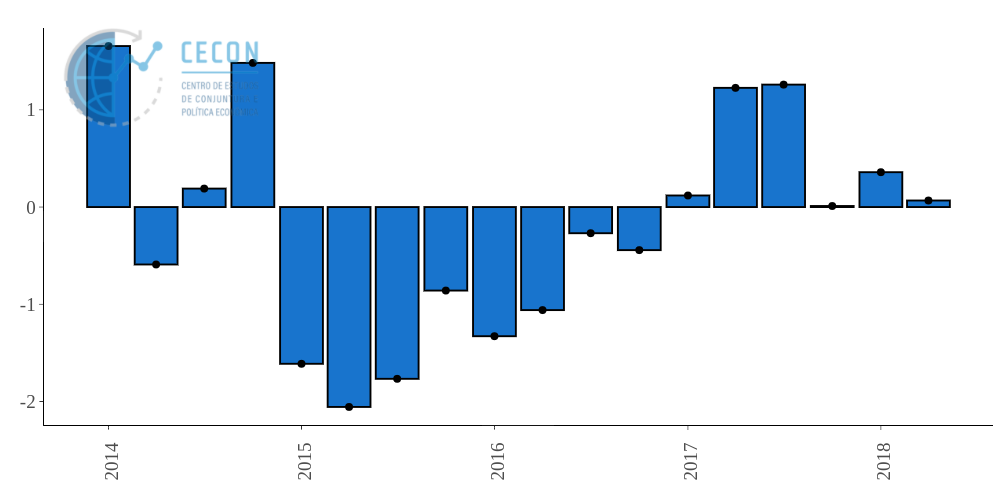
\includegraphics[width=1\linewidth]{Grafico_CFam} \end{center}

\subsection{Consumo do Governo}\label{consumo-do-governo}

\begin{center}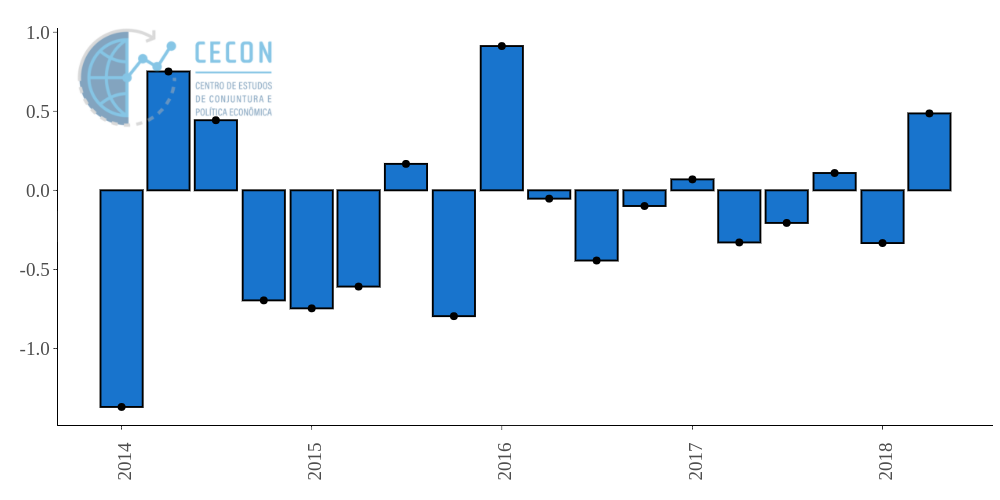
\includegraphics[width=1\linewidth]{Grafico_CGov} \end{center}

\subsection{Formação Bruta de Capital
Fixo}\label{formacao-bruta-de-capital-fixo}

\begin{center}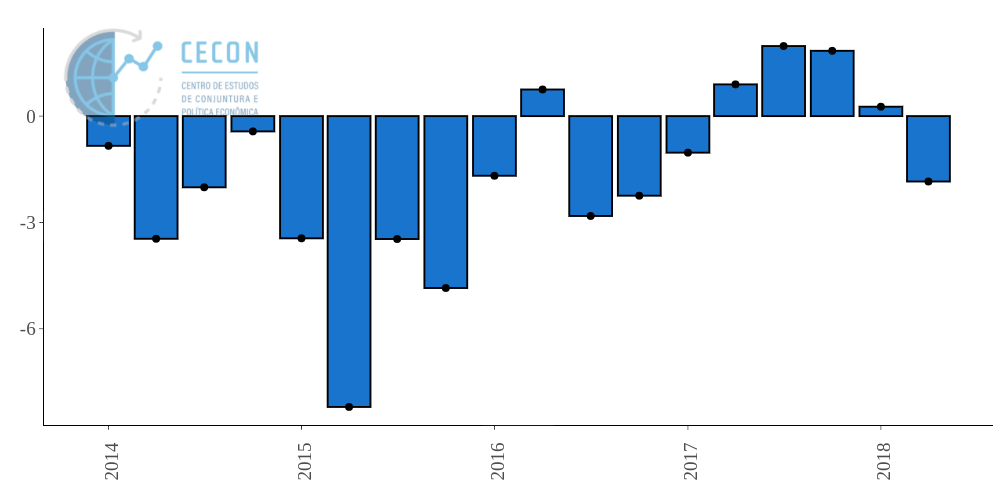
\includegraphics[width=1\linewidth]{Grafico_FBCF} \end{center}

\subsection{Exportação}\label{exportacao}

\begin{center}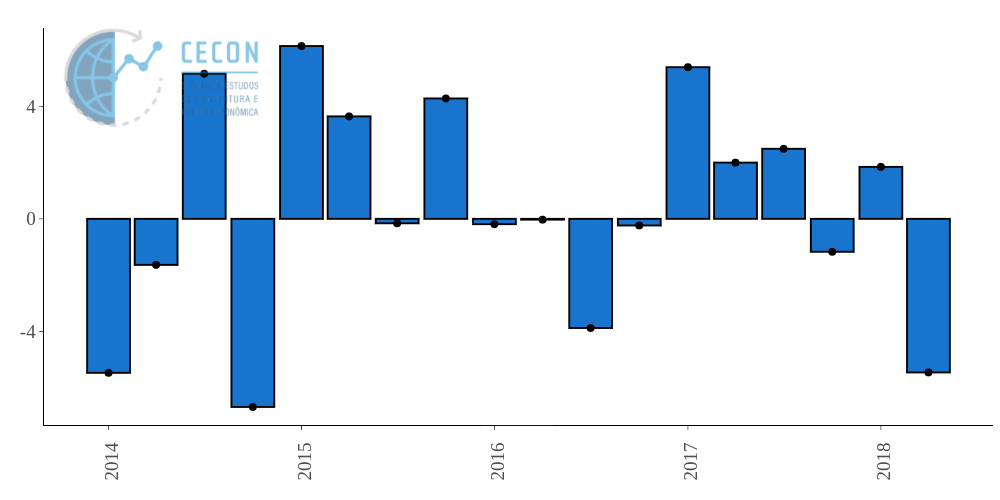
\includegraphics[width=1\linewidth]{Grafico_Export} \end{center}

\subsection{Importação}\label{importacao}

\begin{center}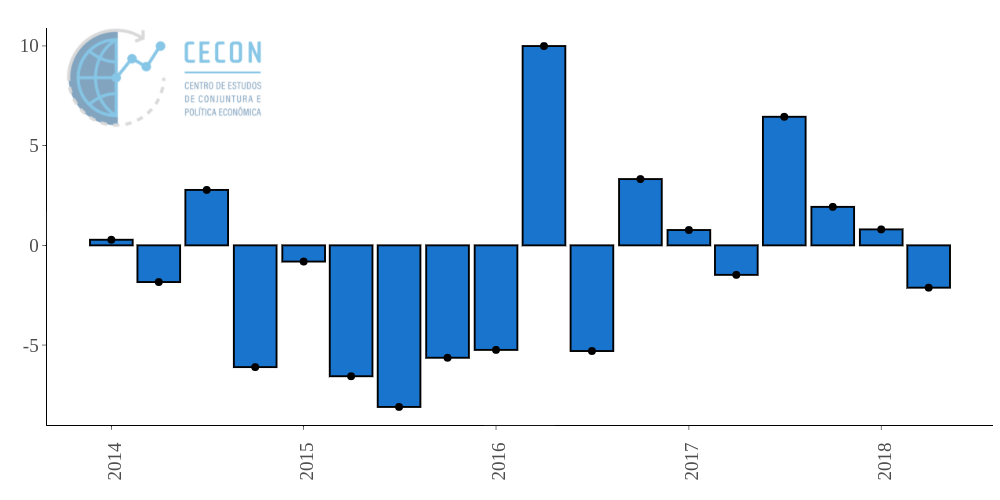
\includegraphics[width=1\linewidth]{Grafico_Import} \end{center}

\subsection{Saldo da Balança
Comercial}\label{saldo-da-balanca-comercial}

\begin{center}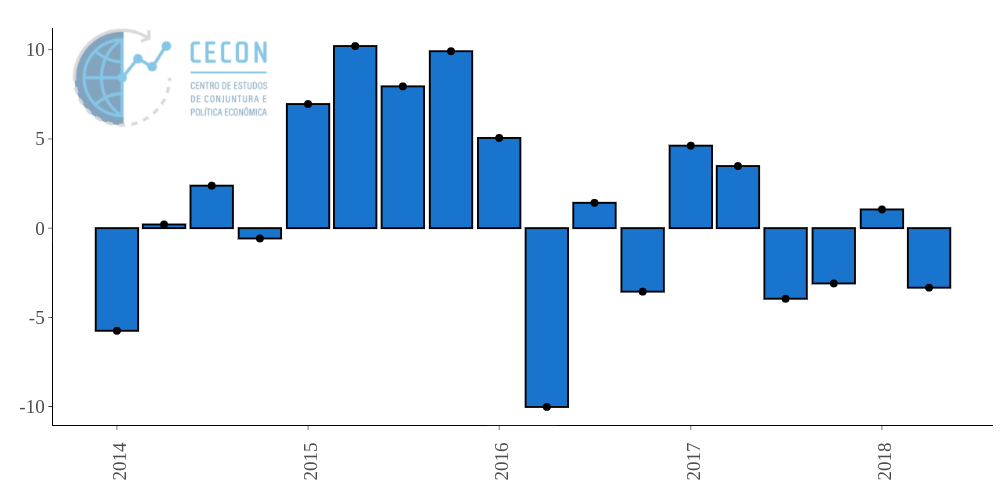
\includegraphics[width=1\linewidth]{Grafico_Bal_Comerc} \end{center}

\section{Todo}\label{todo}

\subsection{TODOs}\label{todos}

\begin{itemize}
\tightlist
\item
  Checar taxa de decomposição
\item
  Substituir na pasta 20182TPIB
\item
  Criar pasta github
\item
  Criar instruções de uso
\end{itemize}


\end{document}
